%%%%%%%%%%%%%%%%%%%%%%%%%%
\chapter{Constraints and Terminologies}
\label{chap::CONSTRAINTS AND TERMINOLOGIES}
%%%%%%%%%%%%%%%%%%%%%%%%%%

\baselineskip=26pt
\hspace{5mm}
In this section, the capacity constraint in bus-pin-aware bus-driven floorplanning
are defined, followed by the introduction of the terminologies
used in this paper.

\begin{figure}[htb]
  \centering
    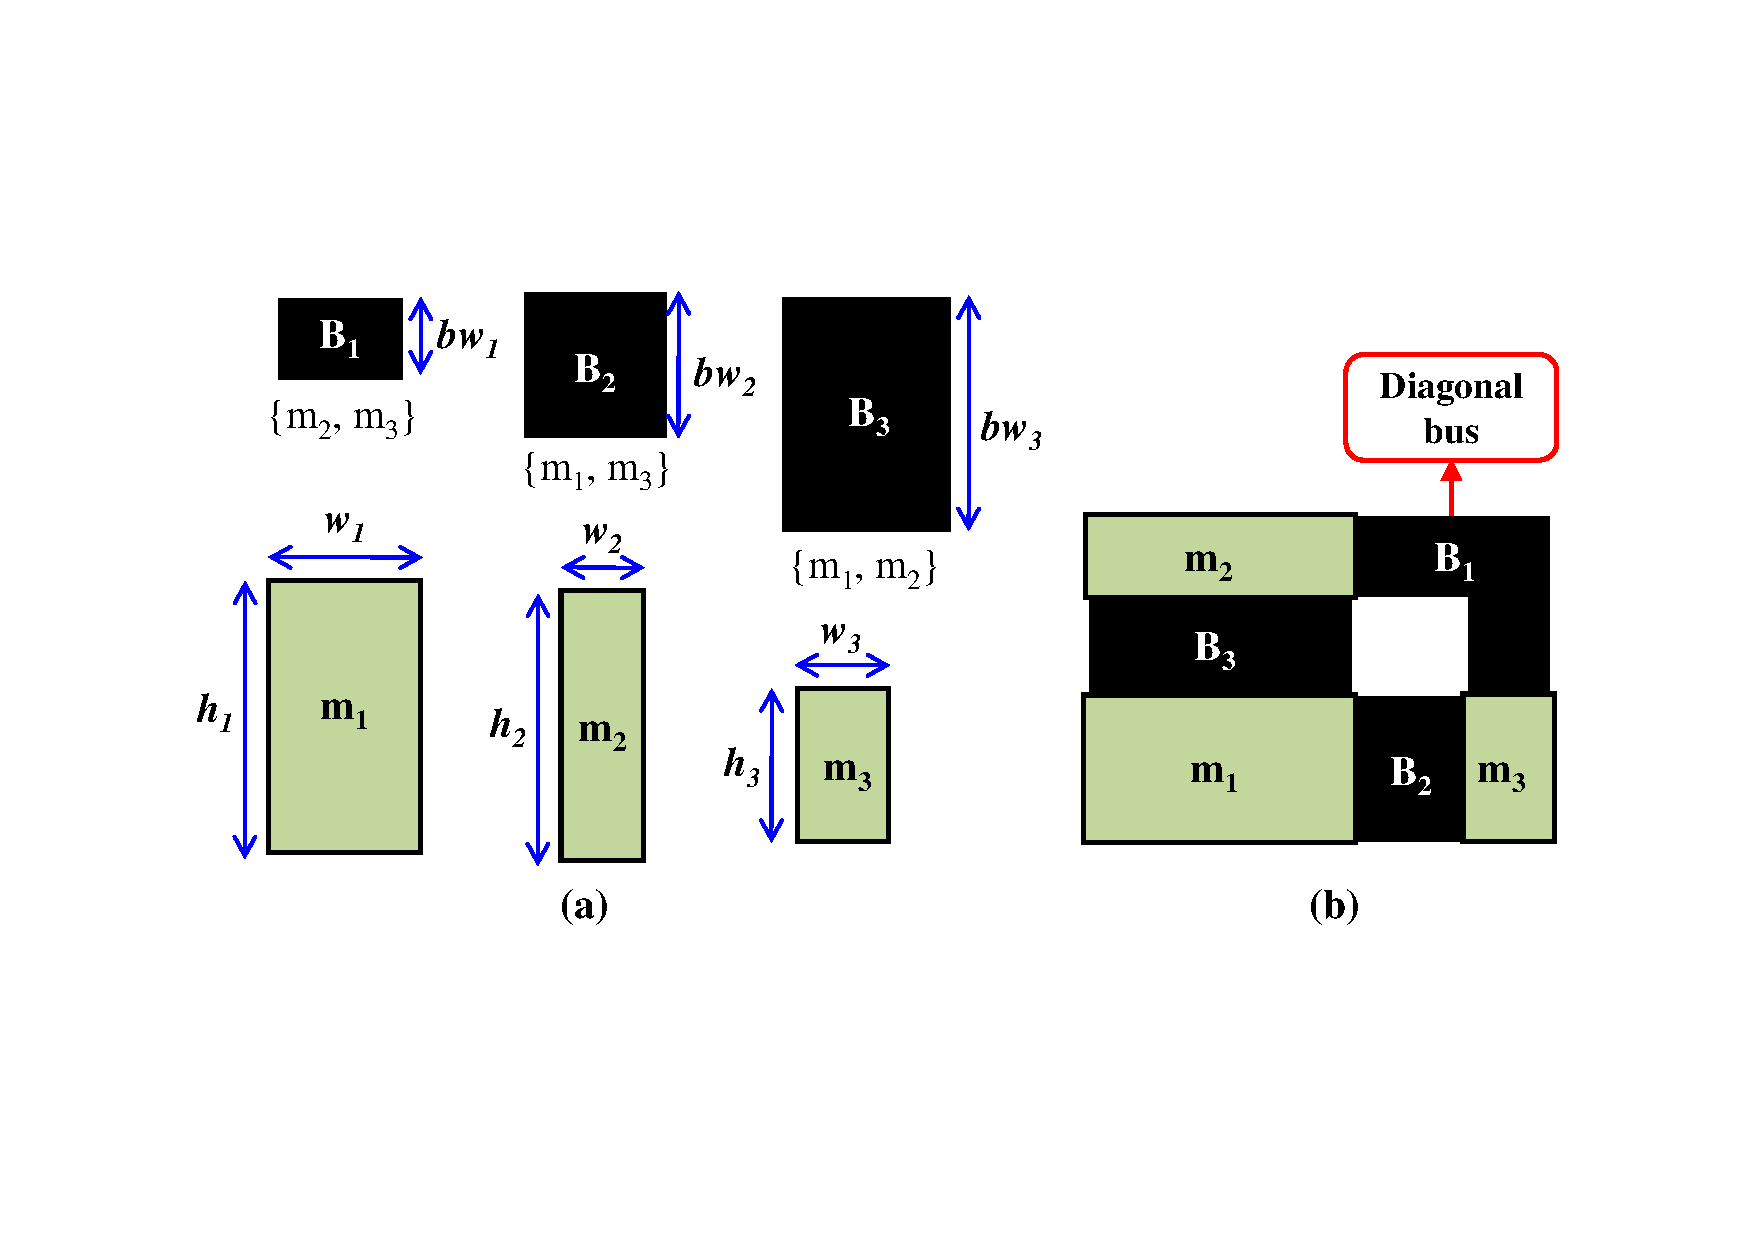
\includegraphics[width=12cm]{Fig/capacity.pdf}
    %\centerline{\psfig{figure=Fig/capacity.eps, width=12cm}}
  \caption{
      (a) Capacity constraint. (b) A routable solution under the capacity
      constraint.
   }
  \label{fig::capacity}
\end{figure}

Capacity constraint is illustrated in Figure~\ref{fig::capacity}
(a). There are three buses $B_1$ = \{$m_2$, $m_3$\}, $B_2$ = \{$m_1$, $m_3$\}, and
$B_3$ = \{$m_1$, $m_2$\}, moreover, three modules $m_1$, $m_2$, and $m_3$ are
placed on the floorplan. $bw_i$ is the bus width of bus
$B_i$, and the width and height of each module $m_i$ are
denoted by $w_i$ and $h_i$, respectively.

Since the capacity of each module is limit, some modules can be passed with only
one bus at the same direction. For instance, $bw_2$ + $bw_3 >$
max($w_1$, $h_1$), therefore, the capacity of the module $m_1$ is
not enough for both buses $B_2$ and $B_3$ to pass through.

Compared with existing bus-driven floorplanning algorithms which
result in an unroutable solution in this example, we can have a
routable solution by exploring the diagonal connection between
different modules in Figure~\ref{fig::capacity} (b). The modified
graph coloring algorithm is proposed to assign the bus components
of the diagonal bus $B_1$ to the same layer such that no extra via
is required at the bend of the bus $B_1$.

\begin{figure}[htb]
  \centering
    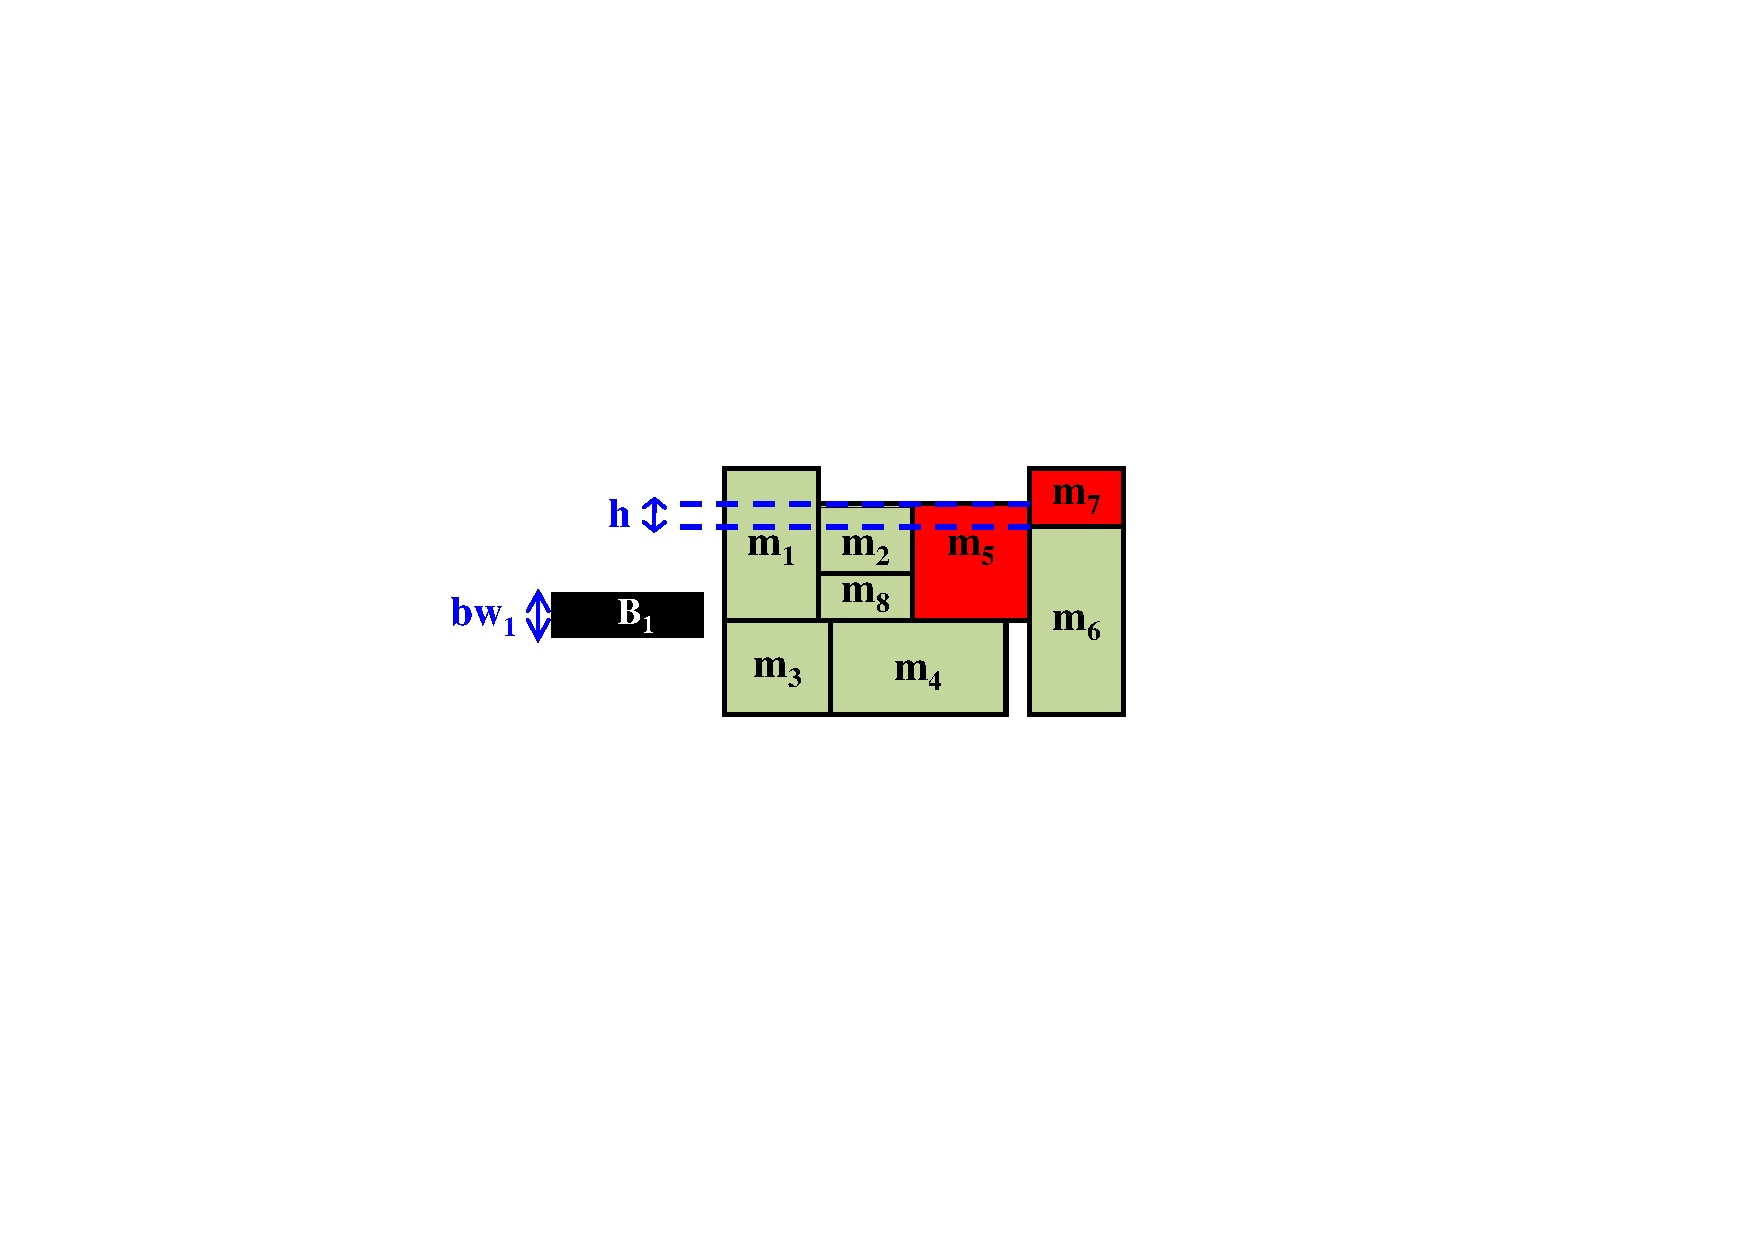
\includegraphics[width=7cm]{Fig/vertical_overlapping.pdf}
    %\centerline{\psfig{figure=Fig/vertical_overlapping.eps, width=7cm}}
     \caption{
      Vertical overlapping.
   }
  \label{fig::vertical_overlapping}
\end{figure}

Another constraint is vertical overlapping as shown in
Figure~\ref{fig::vertical_overlapping}, the bus width of $B_1$
is $bw_1$ and it connects two modules $m_5$ and $m_7$, the
overlapped range between two modules is $h$. If $h < bw_1$, then
it has no sufficient space for the bus $B_1$ to pass through that
the vertical overlapping constraint is violated, thus, the coordinate
of the module $m_5$ must be adjusted to increase the overlapped range.

Terminologies used in this paper are introduced as follows:

{\bf Definition 1}: A \textbf{\textit{bus pin}} of an n-bit bus
consists of n pins. The bits of each bus pin are arranged
monotonically from the Least Significant Bit (LSB) to the MSB,
and are equally spaced. The MSB bit is marked with black color
in all figures of this paper. A bus pin is
oriented horizontally or vertically. For example, the bus pins
$BP_1$, $BP_2$, and $BP_6$ are oriented horizontally, and the bus
pins $BP_3$, $BP_4$, and $BP_5$ are oriented vertically in
Figure~\ref{fig::bus_pin_flipping} (a).

\begin{figure}[htb]
  \centering
    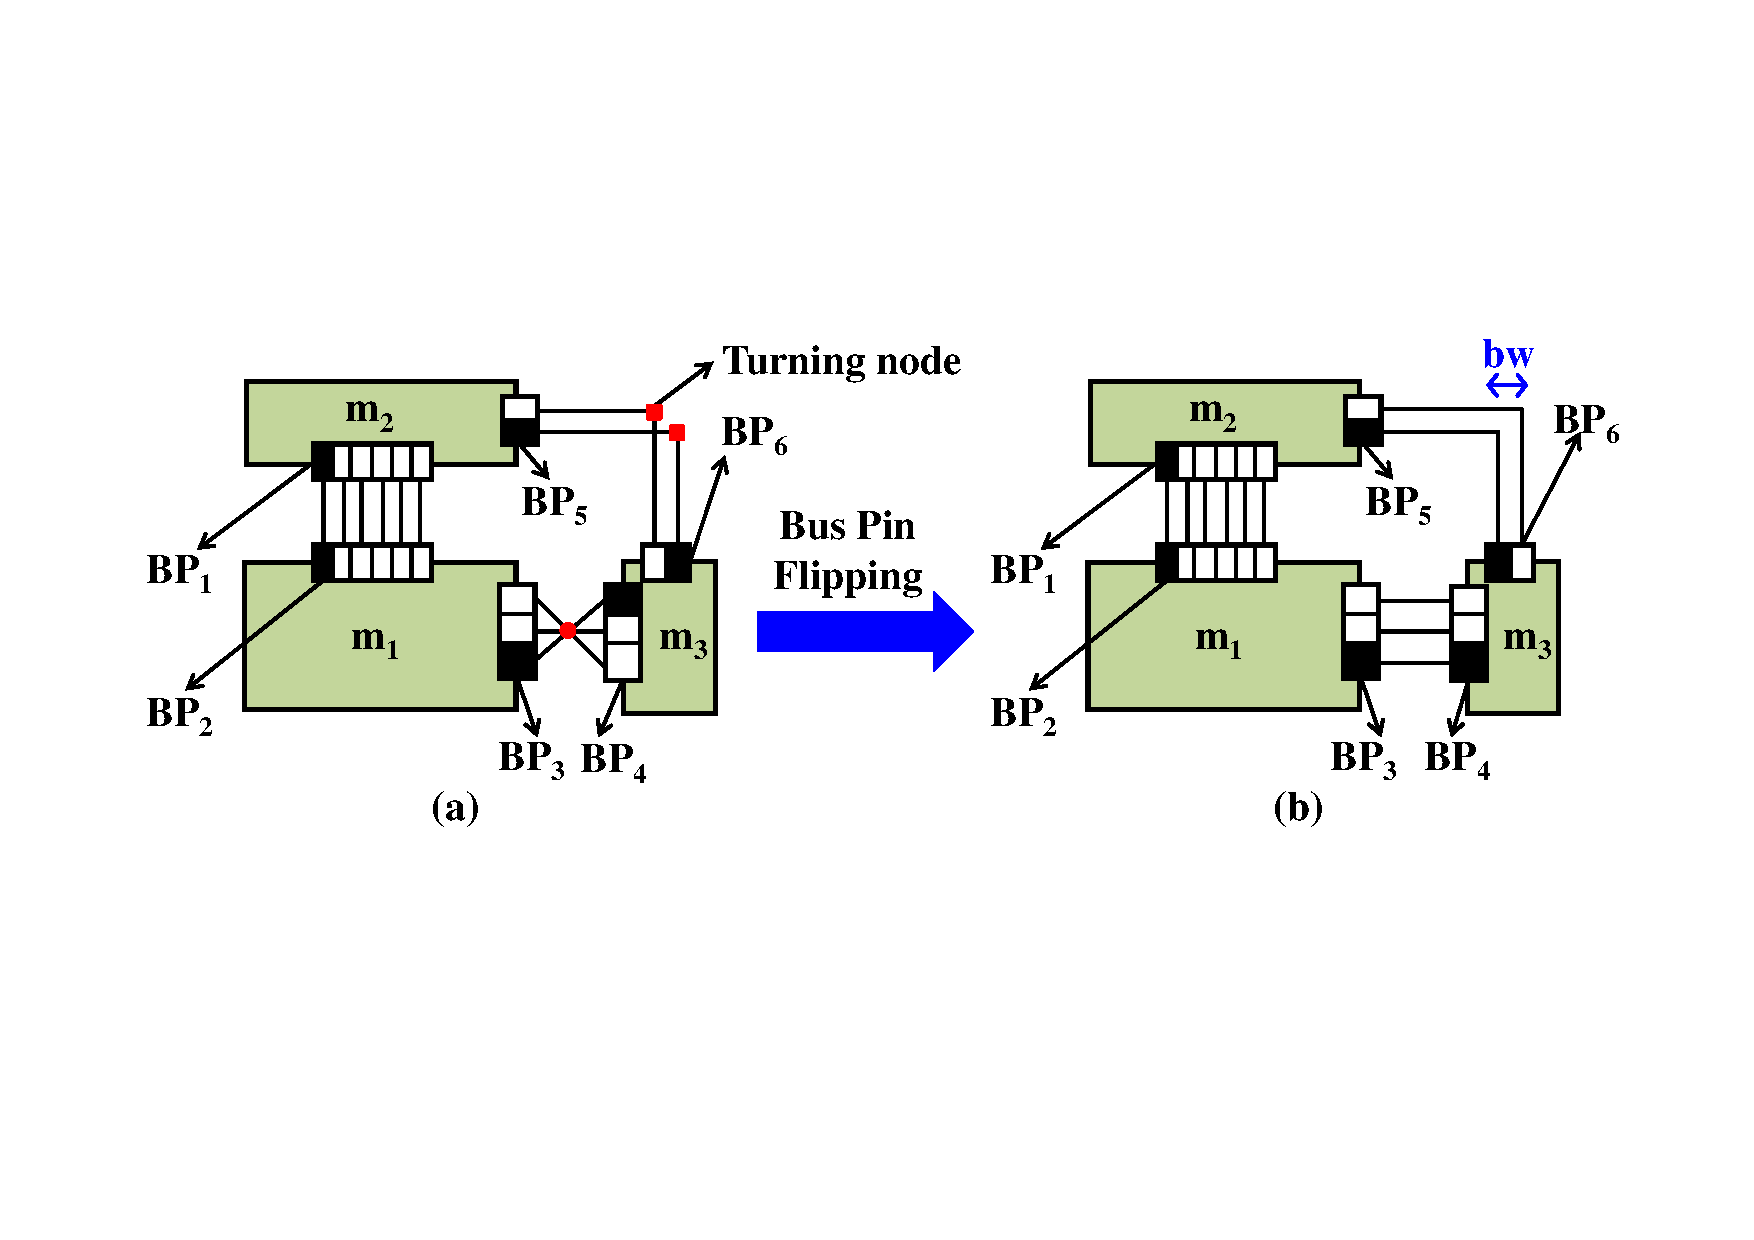
\includegraphics[width=13cm]{Fig/bus_pin_flipping.pdf}
    %\centerline{\psfig{figure=Fig/bus_pin_flipping.eps, width=13cm}}
     \caption{
      Bus pin flipping.
   }
  \label{fig::bus_pin_flipping}
\end{figure}

{\bf Definition 2}: The \textbf{\textit{position of the bus pin}}
is the position of the bus pin on the module, it can be placed on
one of the four boundaries of the modules. For example, the bus pin
$BP_1$ is placed on the lower boundary of the module $m_2$ in
Figure~\ref{fig::bus_pin_flipping} (a).

{\bf Definition 3}:  \textbf{\textit{Turning nodes}} denote the
bends of the buses and they are connected with the horizontal and
vertical buses. For example, there are two turning nodes at the
bend of the bus connecting the bus pins $BP_5$ and $BP_6$ in the
Figure~\ref{fig::bus_pin_flipping} (a).

{\bf Definition 4}: The \textbf{\textit{orientation of the bus
pin}} is defined as the direction from the LSB to the MSB. For
example, the orientation of the bus pin $BP_1$ is from east to west,
and the orientation of the bus pin $BP_3$ is from north to south in
Figure~\ref{fig::bus_pin_flipping}(a). All possible orientations
for the bus pins and the turning nodes are listed in
Figure~\ref{fig::orientation_direction}.

\begin{figure}[htb]
  \centering
    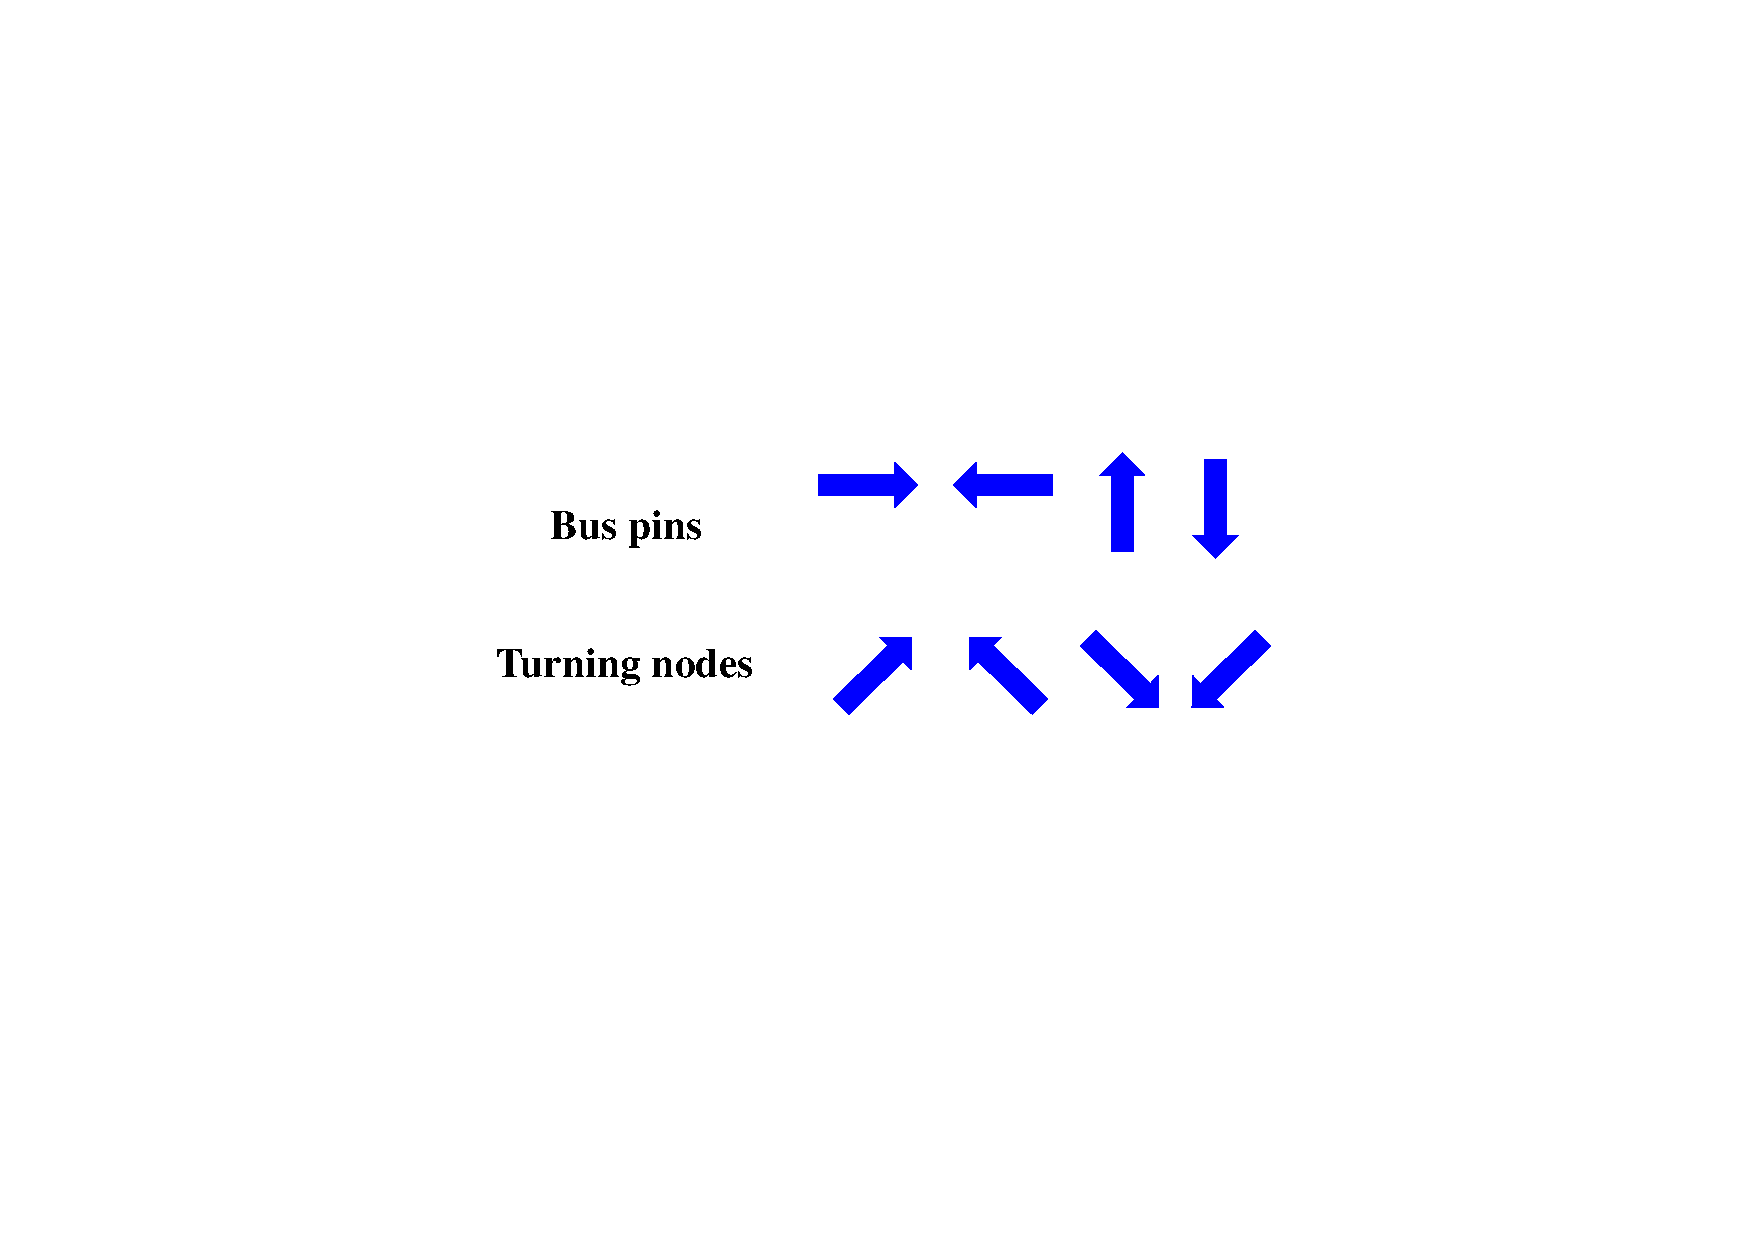
\includegraphics[width=7cm]{Fig/orientation_direction.pdf}
    %\centerline{\psfig{figure=Fig/orientation_direction.eps, width=7cm}}
     \caption{
      The possible orientation directions.
   }
  \label{fig::orientation_direction}
\end{figure}

{\bf Definition 5}: \textbf{\textit{Bus pin flipping}} is used to
change the orientation of the bus pins. In
Figure~\ref{fig::bus_pin_flipping} (a), the orientation of the bus pin
$BP_3$ is from north to south and the orientation of the bus pin
$BP_4$ is from south to north. Since their orientation is opposite and
they are connected with one horizontal bus, the bus twisting makes the signal
wires cross at a point. Furthermore, the bus pin $BP_5$ and $BP_6$ are
connected with a diagonal bus, the orientation of the bus pin $BP_5$ is from
north to south and the orientation of the bus pin $BP_6$ is from west
to east, two extra vias is required at the turning nodes as shown in Figure~\ref{fig::bus_pin_flipping} (a).
All the above problems can be solved
by simply applying bus pin flipping on the bus pins $BP_4$ and $BP_6$.
The result after bus flipping is shown in Figure~\ref{fig::bus_pin_flipping} (b).

{\bf Definition 6}: Wirelength $``$\textbf{\textit{deviation}}$"$
represents the driver-load wirelength difference among all bus bits.
Different choices of the orientations at the bus pins and
turning nodes may cause different driver-load wirelength among all
bits. In this paper, we only need to minimize the wirelength
difference between MSB and LSB of the bus because the wirelength
of all other bits can be linearly interpolated by it. The MSB-LSB
wirelength deviation could be expressed by

\begin{eqnarray}
dev_{len} = | len(MSB) - len(LSB)|
\end{eqnarray}

A turning node can contribute $-$D, 0 or $+$D to the MSB-LSB
wirelength difference, where D = 2$\times$$BW$ and $BW$ is the bus width.
Accumulating the turning node contributions along the path from
the driver to the load of the bus provides $dev_{len}$ at the
load. Figure~\ref{fig::bus_pin_flipping} illustrates the different
deviation results from the different choices at the turning nodes.
In Figure~\ref{fig::bus_pin_flipping} (b), the deviation from the
bus pin $BP_5$ to the bus pin $BP_6$ is $-$D, while in
Figure~\ref{fig::bus_pin_flipping} (a) is 0, but it needs two
extra vias at the turning nodes. Therefore, it is hard to
optimize the total deviation with no extra vias are used at the
turning nodes.
